\documentclass[11pt]{book}

%%%%%%%%%%%%%%Include Packages%%%%%%%%%%%%%%%%%%%%%%%%%%
\usepackage{xcolor}
\usepackage{mathtools}
\usepackage[legalpaper, total={6in, 8in}, margin=1.25in]{geometry}
\usepackage{amsmath}
\usepackage{amssymb}
\usepackage{paralist}
\usepackage{rsfso}
\usepackage{amsthm}
\usepackage{wasysym}
\usepackage[inline]{enumitem}   
\usepackage{hyperref}
\usepackage{tocloft}
\usepackage{wrapfig}
\usepackage{titlesec}
\usepackage{colortbl}
\usepackage{stackengine} 
\usepackage{csvsimple}
\usepackage{listings}
%%%%%%%%%%%%%%%%%%%%%%%%%%%%%%%%%%%%%%%%%%%%%%%%%%%%%%%%



%%%%%%%%%%%%%%%Code%%%%%%%%%%%%%%%%%%%%%%%%%%%%%%%%%%%%%
\definecolor{codegreen}{rgb}{0,0.6,0}
\definecolor{codegray}{rgb}{0.5,0.5,0.5}
\definecolor{codepurple}{rgb}{0.58,0,0.82}
\definecolor{backcolour}{rgb}{0.95,0.95,0.92}

\lstdefinestyle{mystyle}{
    backgroundcolor=\color{backcolour},   
    commentstyle=\color{codegreen},
    keywordstyle=\color{magenta},
    numberstyle=\tiny\color{codegray},
    stringstyle=\color{codepurple},
    basicstyle=\ttfamily\footnotesize,
    breakatwhitespace=false,         
    breaklines=true,                 
    captionpos=b,                    
    keepspaces=true,                 
    numbers=left,                    
    numbersep=5pt,                  
    showspaces=false,                
    showstringspaces=false,
    showtabs=false,                  
    tabsize=2
}
%%%%%%%%%%%%%%%%%%%%%%%%%%%%%%%%%%%%%%%%%%%%%%%%%%%%%%%%




%%%%%%%%%%%%%%%Chapter Setting%%%%%%%%%%%%%%%%%%%%%%%%%%
\definecolor{gray75}{gray}{0.75}
\newcommand{\hsp}{\hspace{20pt}}
\titleformat{\chapter}[hang]{\Huge\bfseries}{\thechapter\hsp\textcolor{gray75}{$\mid$}\hsp}{0pt}{\Huge\bfseries}
%%%%%%%%%%%%%%%%%%%%%%%%%%%%%%%%%%%%%%%%%%%%%%%%%%%%%%%%

%%%%%%%%%%%%%%%%%Theorem environments%%%%%%%%%%%%%%%%%%%
\newtheoremstyle{break}
  {\topsep}{\topsep}%
  {\itshape}{}%
  {\bfseries}{}%
  {\newline}{}%
\theoremstyle{break}
\theoremstyle{break}
\newtheorem{axiom}{Axiom}
\newtheorem{thm}{Theorem}[section]
\renewcommand{\thethm}{\arabic{section}.\arabic{thm}}
\newtheorem{lem}{Lemma}[thm]
\newtheorem{prop}[lem]{Proposition}
\newtheorem{corL}{Corollary}[lem]
\newtheorem{corT}[lem]{Corollary}
\newtheorem{defn}{Definition}[corL]
\newenvironment{indEnv}[1][Proof]
  {\proof[#1]\leftskip=1cm\rightskip=1cm}
  {\endproof}
%%%%%%%%%%%%%%%%%%%%%%%%%%%%%%%%%%%%%%%%%%%%%%%%%%%%%%


%%%%%%%%%%%%%%%%%%%%%%%Integral%%%%%%%%%%%%%%%%%%%%%%%
\def\upint{\mathchoice%
    {\mkern13mu\overline{\vphantom{\intop}\mkern7mu}\mkern-20mu}%
    {\mkern7mu\overline{\vphantom{\intop}\mkern7mu}\mkern-14mu}%
    {\mkern7mu\overline{\vphantom{\intop}\mkern7mu}\mkern-14mu}%
    {\mkern7mu\overline{\vphantom{\intop}\mkern7mu}\mkern-14mu}%
  \int}
\def\lowint{\mkern3mu\underline{\vphantom{\intop}\mkern7mu}\mkern-10mu\int}
%%%%%%%%%%%%%%%%%%%%%%%%%%%%%%%%%%%%%%%%%%%%%%%%%%%%%%



\newcommand{\R}{\mathbb{R}}
\newcommand{\N}{\mathbb{N}}
\newcommand{\Z}{\mathbb{Z}}
\newcommand{\Q}{\mathbb{Q}}
\newcommand{\C}{\mathbb{C}}
\newcommand{\T}{\mathcal{T}}
\newcommand{\M}{\mathcal{M}}
\newcommand{\Symm}{\text{Symm}}
\newcommand{\Alt}{\text{Alt}}
\newcommand{\Int}{\text{Int}}
\newcommand{\Bd}{\text{Bd}}
\newcommand{\Power}{\mathcal{P}}
\newcommand{\ee}[1]{\cdot 10^{#1}}
\newcommand{\spa}{\text{span}}
\newcommand{\sgn}{\text{sgn}}
\newcommand{\degr}{\text{deg}}
\newcommand{\pd}{\partial}
\newcommand{\that}[1]{\widetilde{#1}}
\newcommand{\lr}[1]{\left(#1\right)}
\newcommand{\vmat}[1]{\begin{vmatrix} #1 \end{vmatrix}}
\newcommand{\bmat}[1]{\begin{bmatrix} #1 \end{bmatrix}}
\newcommand{\pmat}[1]{\begin{pmatrix} #1 \end{pmatrix}}
\newcommand{\rref}{\xrightarrow{\text{row\ reduce}}}
\newcommand{\txtarrow}[1]{\xrightarrow{\text{#1}}}
\newcommand\oast{\stackMath\mathbin{\stackinset{c}{0ex}{c}{0ex}{\ast}{\Circle}}}


\newcommand{\note}{\color{red}Note: \color{black}}
\newcommand{\remark}{\color{blue}Remark: \color{black}}
\newcommand{\example}{\color{green}Example: \color{black}}
\newcommand{\exercise}{\color{green}Exercise: \color{black}}

%%%%%%%%%%%%%%%%%%%%%%Roman Number%%%%%%%%%%%%%%%%%%%%%%%
\makeatletter
\newcommand*{\rom}[1]{\expandafter\@slowromancap\romannumeral #1@}
\makeatother
%%%%%%%%%%%%%%%%%%%%%%%%%%%%%%%%%%%%%%%%%%%%%%%%%%%%%%%%%

%%%%%%%%%%%%table of contents%%%%%%%%%%%%%%%%%%%%%%%%%%%%
\setlength{\cftchapindent}{0em}
\cftsetindents{section}{2em}{3em}

\renewcommand\cfttoctitlefont{\hfill\huge\bfseries}
\renewcommand\cftaftertoctitle{\hfill\mbox{}}

\setcounter{tocdepth}{2}
%%%%%%%%%%%%%%%%%%%%%%%%%%%%%%%%%%%%%%%%%%%%%%%%%%%%%%%%%


%%%%%%%%%%%%%%%%%%%%%Footnotes%%%%%%%%%%%%%%%%%%%%%%%%%%%
\newcommand\blfootnote[1]{%
  \begingroup
  \renewcommand\thefootnote{}\footnote{#1}%
  \addtocounter{footnote}{-1}%
  \endgroup
}
%%%%%%%%%%%%%%%%%%%%%%%%%%%%%%%%%%%%%%%%%%%%%%%%%%%%%%%%%

%%%%%%%%%%%%%%%%%%%%%Section%%%%%%%%%%%%%%%%%%%%%%%%%%%%%
\makeatletter
\def\@seccntformat#1{%
  \expandafter\ifx\csname c@#1\endcsname\c@section\else
  \csname the#1\endcsname\quad
  \fi}
\makeatother
%%%%%%%%%%%%%%%%%%%%%%%%%%%%%%%%%%%%%%%%%%%%%%%%%%%%%%%%%

%%%%%%%%%%%%%%%%%%%%%%%%%%%%%%%%%%%Enumerate%%%%%%%%%%%%%%
\makeatletter
% This command ignores the optional argument 
% for itemize and enumerate lists
\newcommand{\inlineitem}[1][]{%
\ifnum\enit@type=\tw@
    {\descriptionlabel{#1}}
  \hspace{\labelsep}%
\else
  \ifnum\enit@type=\z@
       \refstepcounter{\@listctr}\fi
    \quad\@itemlabel\hspace{\labelsep}%
\fi}
\makeatother
\parindent=0pt
%%%%%%%%%%%%%%%%%%%%%%%%%%%%%%%%%%%%%%%%%%%%%%%%%%%%%%%%%%


\begin{document}

	\begin{titlepage}
		\begin{center}
			\vspace*{1cm}
			\Huge \color{red}
				\textbf{Lab 1 Report}\\
			\vspace{0.5cm}			
			\Large \color{black}
				Math 391 - Introduction to Modern Physics Lab\\
				Professor Wayne Lau\\	
				University of Michigan\\
			\vspace{3cm}

			
\includegraphics[scale=1.16]{hmm.pdf}
			
			
			\vspace{5cm}
			\LARGE
				\textbf{Jinyan Miao}\\
				\hfill\break
				\LARGE Fall 2022\\
			\vspace{1cm}

		\vspace*{\fill}
		\end{center}			
	\end{titlepage}


\newpage
\tableofcontents
\addtocontents{toc}{~\hfill\textbf{Page}\par}


\setcounter{chapter}{1}
\chapter*{Lab 1 - Statistics}
\section{Introduction}

Statistics methods are important for analyzing real-world observations and making reliable interpretations of experimental data. Since many topics in physics involve analyzing experimental data and generalizing laws of physics through statistical interpretation, a good background in statistics will help us to start a career in physics, and other subjects in the STEM field. Lab 1 in Physics 391 is designed to help us to understand the statistical limitation of using sample distribution to approximate population distribution. We collect sets of data for coin tossing, dice rolling, and salt counting, then we compare our observations with the theoretically expected values. The comparisons will focus on the sample mean and sample variance, and through those comparisons, we can get a deeper understanding of how the sample mean and variance can be used to interpret the population distribution. We will also find the conditions required for approximating a probability distribution using a normal distribution. 

\hfill\break
\hfill\break
\section{Experimental setup and data collection}
Lab 1 of Physics 391 consists of three sub-experiments:
\begin{enumerate}
\item The first experiment is coin tossing. 10 coins (pennies) are placed in a plastic champagne flute, we vigorously shake the cup and dump the coins into a tray, then count the number of heads that appear on top. The coin tossing procedure is performed 50 times, and a set of data is collected, indicating the number of heads each time. In this experiment, the coins are assumed to be fair, that is the probability of getting a head for each coin is exactly 1/2.
\item  The second experiment is dice rolling. 2 dice, each has 6 faces and the faces are numbered from 0 to 5. The two dice are rolled 50 times. A set of data is collected, indicating the sum of the two dice for each roll. In this experiment, the dice are assumed to be fair, that is the probability of getting each face of a dice is exactly 1/6. 
\item The third experiment is salt counting. We measure the number of 
counts of the radioactive decay event recorded by the Spectrum Techniques ST360 Geiger counter system when exposed to canisters of salt for a duration of 8 seconds. We collect two sets of data in this experiment, the first set of data contains the counts indicated by the Geiger counter when it is surrounded by 6 canisters of table salt (NaCl), and the second set of data contains the counts indicated by the Geiger counter when it is surrounded by 6 canisters of sodium-free salt substitute (KCl). 50 counts are recorded for each type of salts. In this experiment, we are interested in determining whether KCl is more radioactive than the average room background. If KCl is more radioactive, we expect to see more decay events occur in 8 seconds for KCl than that for NaCl.
\end{enumerate}

The experiment collected data is attached at the end of this text.
\newpage

\section{Visualizing the data}
For the coin tossing experiment, the following figure (Fig 1.1) plots the total count of the number of heads in ten flips.
\begin{center}
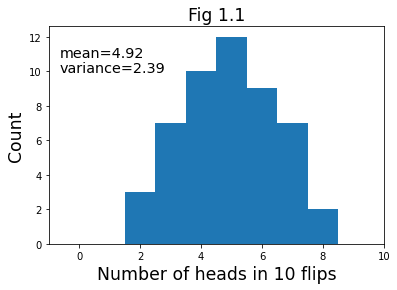
\includegraphics[scale=0.5]{Fig1.1.png}
\end{center}
\hfill\break
For the dice rolling experiment, the following figure (Fig 1.2) plots the count of the sum of the two dice.
\begin{center}
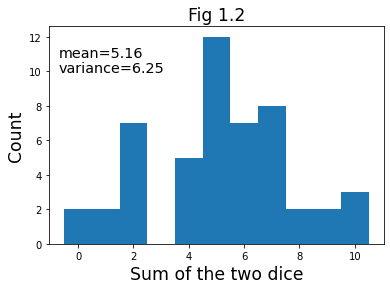
\includegraphics[scale=0.5]{Fig1.2.png}
\end{center}
\hfill\break
For the salt counting experiment, the figure on the left (Fig 1.3a) plots the count recorded by the Geiger counter for the KCl in the 50 8-seconds intervals, and the figure on the right (Fig 1.3b) plots the count recorded by the Geiger counter for the background (NaCl) in the 50 8-seconds intervals.
\begin{center}
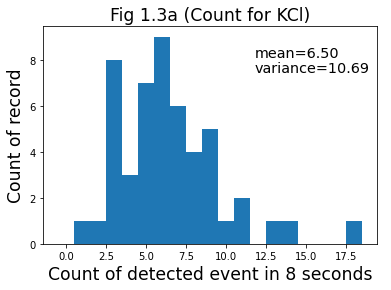
\includegraphics[scale=0.5]{Fig1.3a.png}\qquad
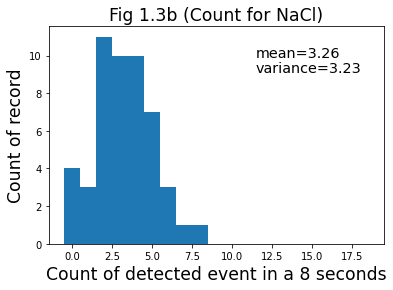
\includegraphics[scale=0.5]{Fig1.3b.png}
\end{center}
\hfill\break

The following table display some important statistics of the collected data. Quantities are calculated using formulas provided on the Physics 391 Lab Manual. 
\begin{center}
\begin{tabular}{|c|c|c|c|c|}
\hline 
Experiment & Sample Mean & Sample Variance & Population Mean & Population Variance \\
\hline
Coin tossing & $4.92$ & $2.39$ & $5.00$ & $2.50$\\
\hline 
Dice rolling & $5.16$ & $6.25$ & $5.00$ & $5.83$\\
\hline
Count for KCl & $6.50$ & $10.69$ & $-$ & $-$\\
\hline
Count for NaCl & $3.26$ & $3.23$ & $-$ & $-$\\
\hline
\end{tabular}
\end{center}

\newpage
Here we note that the population means and population variance of the count of salts are unknown. Since, according to equation (8) and equation (16) from the Lab Manual, the calculation of the variance of sample means and variance of sample variance involves the population variance, we are not able to directly calculate those for the count of salts experiment. However, we can use the sample variance to estimate the population variance for the count of salts, in which case we can substitute the population variance by sample variance to calculate the variance of sample means and the variance of sample variance for the count of salts experiment. And we also do a similar calculation for the coins experiment and the dice experiment just for comparison. 
\begin{center}
\begin{tabular}{|c|c|c|}
\hline 
${\ }$ & Variance of Sample Mean & Variance of Sample Variance \\
Experiment & (using population variance)& (using population variance) \\
\hline
Coin tossing & $0.05$ & $0.23$ \\
\hline 
Dice rolling & $0.12$ & $0.96$ \\
\hline
\end{tabular}\\
\hfill\break
\hfill\break
\begin{tabular}{|c|c|c|}
\hline 
${\ }$ & Variance of Sample Mean & Variance of Sample Variance \\
Experiment & (using sample variance) &  (using sample variance) \\
\hline
Coin tossing & $0.05$ & $0.21$ \\
\hline 
Dice rolling & $0.13$ & $1.13$ \\
\hline
Count for KCl & $0.21$ & $4.88$ \\
\hline
Count for NaCl & $0.06$ & $0.49$ \\
\hline
\end{tabular}
\end{center}

\hfill\break
\hfill\break
\hfill\break


\section{Analyzing the data}
In this section, we will analyze the result of each experiment separately.\\



For the coin tossing experiment, the sample mean we obtained is 4.92 heads per 10 flips, compared to the population mean of 5.00 heads per 10 flips. The variance of sample means, calculated using population variance, is 0.05, and hence the standard deviation of the sample means is around 0.22. Here we see that the difference between the sample mean and the population mean is only 0.08, which is less than 1 standard deviation of the sample means. This shows that our sample mean is within the statistical expected dispersion from the population mean. On the other hand, the sample variance of our data is 2.39, and the population variance is 2.50, so the difference between the two is 0.11. The variance of the sample variance, calculated using the population variance, is 0.23, so the standard deviation of the sample variance is 0.48.  We see that our sample variance is also less than 1 standard deviation of the sample variance, which indicates that our sample variance is within the statistical expected dispersion from the population variance. We also notice that the difference in the variance of sample means calculated using the two methods, using the sample variance and using the population variance, is small enough to be neglected, and the difference in the variance of the sample variance calculated using the two methods (0.23 versus 0.21) is also statistically insignificant. These results indicate that our sample variance is a reasonable estimation of the population variance, and also suggest that our experimental results are within statistical expectation. \\


For the dice rolling experiment. The sample mean value of the sum of the two dice is 5.16, compared to the population mean of 5.00. The variance of sample means, calculated using the population variance, is 0.12, and hence the standard deviation of the sample means is around 0.35. Therefore, the difference between the sample mean and the population mean is within 1 standard deviation, indicating that our sample mean is within the statistical expected dispersion from the population mean, and hence our sample mean is a good estimation of the population mean. On the other hand, our sample variance is 6.25, and the population variance is 5.83. The variance of sample variance calculated using the population variance is 0.96, which implies the standard deviation of the sample variance is 0.97. So we conclude that our sample variance is within 1 standard deviation of the sample variance, and hence it is also statistically well-expected. Notice that the variance of the sample means and the variance of the sample variance in this experiment are much greater than that in the coin tossing experiment, and this statistical phenomenon is also illustrated by the shape of the sample distributions in Fig 1.1 and Fig 1.2. The shape of the distribution shown in Fig 1.1 for the coin tossing experiment is narrower than that in Fig 1.2 for the dice rolling experiment. This suggests that, even though we have the same population mean for the two experiments, the distribution of the two experiments is rather different, and we can get insights of the shape of the distribution by examining the population variance. We also see that the variance of sample means calculated using the sample variance is very close to that calculated using the population variance (0.12 versus 0.13), and the difference between the variance of the sample variance calculated using the two methods (0.96 versus 1.13) is also small. Therefore, we conclude that the sample variance in this experiment also serves as a good estimator for the population variance. Furthermore, both the coin tossing experiment and the dice rolling experiment suggest that one can use the sample mean and sample variance to estimate the population mean and population variance when the sample size is large enough, and as a result, the sample variance also predicts the shape of the population distribution as well as the shape of the sample distribution. \\

For the salts counting experiment, we are interested in whether the number of decay events for KCl is greater than that of NaCl. We start by computing the difference in the means of counts, let $X$ denote the dataset of KCl, and let ${Y}$ denote the dataset of NaCl:
$$\Delta = \overline{X} - \overline{Y} = 6.50-3.26 = 3.24$$
When comparing the difference between means, assuming the two datasets are independent of each other, then the variances of the two datasets add, hence we write:
$$\mathbb{V}(X-Y) = \mathbb{V}(X)+\mathbb{V}(Y) = 10.69+3.23 = 13.92 $$
Now we can compute the standard deviation for $X-Y$:
$$\sigma = \sqrt{\mathbb{V}(X-Y)} = \sqrt{ 13.92} = 3.731$$
To determine whether the difference between $X$ and $Y$ is significant, we need to examine the variance of the sample means for $X-Y$:
$$\mathbb{V}\left(\overline{X-Y}\right) = \mathbb{V}\left(\overline{X}\right) + \mathbb{V}\left(\overline{Y}\right) = 0.21+0.06 = 0.27$$
Now we can compute the standard deviation of sample means for $X-Y$:
$$\sigma_d = \sqrt{\mathbb{V}\left(\overline{X-Y}\right)} = \sqrt{0.27} =0.52$$
Here we can perform the 2-sample t-test for the two datasets $X$ and $Y$, and the test statistic $t$ is calculated as the following:
$$ t = \frac{\Delta}{\sigma_{d}} = \frac{3.24}{0.52} = 6.25$$
If the two population distributions for the two sample datasets have the same mean, then one would expect to have $0$ being captured within 3 $\sigma_d$ from $\Delta$. However, the test statistic $t$ indicates that $0$ is 6.25 $\sigma_d$ away from $\Delta$, implying a low probability of equal population means for the count of decay events of the two salts. In particular, denoting means of the population distribution of KCl decay count and NaCl decay count as $\mu(X)$ and $\mu(Y)$, respectively, the one-sided 2-sample t-test statistic suggests that that $p$-value for $\mu(X) > \mu(Y)$ is given by:
$$p\left(\mu(X) > \mu(Y)\right) < 0.0001 < 0.05$$
hence we can reject the null hypothesis that $\mu(X) \not > \mu(Y)$, and we conclude that there is statistical evidence that the population mean of KCl decay event is greater than that of NaCl, which implies that the KCl is more radioactive than the background (NaCl). Furthermore, we want to check how good our variance for $X-Y$ is, which requires us to examine the variance of the sample variance of $X-Y$, that is, we write:
$$\mathbb{V}\left(\mathbb{V}(X-Y)\right) =\mathbb{V}(\mathbb{V}(X)) + \mathbb{V}(\mathbb{V}(Y)) =4.88+0.49=5.37$$ 
so the standard deviation for the variance of $X-Y$ is given by:
$$\sigma_v = \sqrt{\mathbb{V}\left(\mathbb{V}(X-Y)\right)} = \sqrt{5.37} = 2.32$$
compare the value of $\mathbb{V}(X-Y)$ in our experiment, we see that $\sigma_v$ is rather small, hence the value of $\mathbb{V}(X-Y)$ in our experiment is reliable.\\

\newpage
\section{Normal Approximation}
The underlying probability distribution for the coin tossing experiment is in fact a binomial distribution as mentioned in the Lab Manual. Even though the probability distribution for the two-dice rolling experiment is not exactly binomial, a binomial distribution still serves as an adequate approximation for the probability distribution of multi-dice rolling. The underlying probability distribution for the salts counting experiment is the Poisson distribution. On the other hand, by the Central Limit Theorem, both the binomial distribution and the Poisson distribution can be approximated by a normal distribution in many circumstances, say, the sample size is large enough. In this section, we will investigate how normal our sample distributions are.\\


\begin{center}
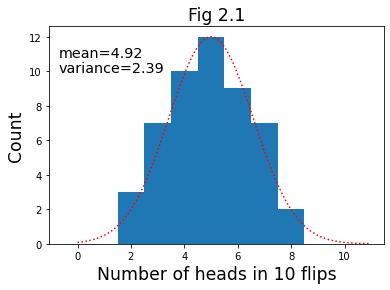
\includegraphics[scale=0.5]{Fig2.1.png}
\end{center}
Fig 2.1 plots the sample distribution of the coin tossing experiment. The red curve is the normal distribution with the population mean and variance of the coin tossing population. The amplitude of the normal distribution curve is set to be the maximum of counts in our sample data. We see that the red curve gives an excellent approximation for the shape of our sample distribution, which suggests that normal distribution is indeed a good approximation for the binomial distribution when the sample size is large enough. The sample size in our experiment is 50.
\hfill\break
\begin{center}
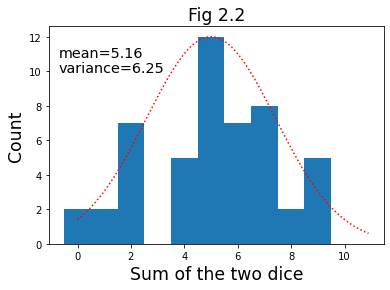
\includegraphics[scale=0.5]{Fig2.2.png}
\end{center}
Fig 2.2 plots the sample distribution of the dice rolling experiment. The red curve is the normal distribution with the population mean and variance of the sum of the two-dice rolling population. The amplitude of the normal distribution curve is set to be the maximum of sums in our sample data. In our sample distribution, there is no count record at a sum equal to 3, which makes our model appears to be a little bimodel. Nevertheless, the overall shape of our sample distribution is still outlined by the red curve, and we expect that the red curve will give an even better approximation for the sample distribution if we collect more sample data.\\


\hfill\break
\begin{center}
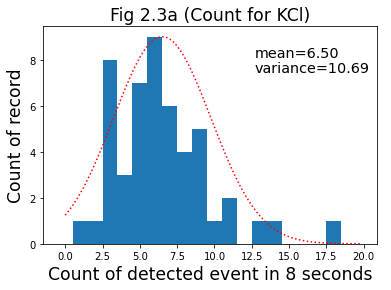
\includegraphics[scale=0.5]{Fig2.3a.png}\qquad
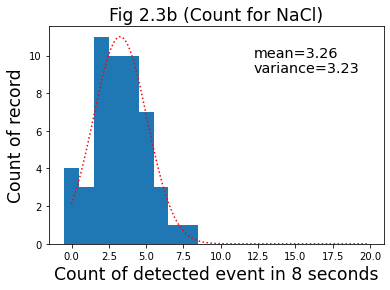
\includegraphics[scale=0.5]{Fig2.3b.png}
\end{center}

Fig 2.3a and 2.3b plot the sample distribution for the salts counting experiment. The red curves in both plots are normal distribution curves generated by using the sample mean and variance, with amplitude defined by the maximum of the count of record. Note that one should have used the population mean and variance to generate the normal distribution, but in our case the population distribution is unknown, and as mentioned above, the sample means and variance give a good approximation for the population means and variance when the sample size is large enough, then using the sample mean and variance to generate the normal distribution curve is adequate in our case. We observe that both sample distributions appear to be skewed to the right, which is one of the natures of our model as we do not have negative counts. The red curves do give an approximation for the shape of our sample distribution, except it does not demonstrate the skewness nature of our model. This result verifies the statistical fact that normal distribution is a good approximation for the Poisson distribution only when the population mean of the underlying Poisson distribution is sufficiently large, in which case the skewness of the sample distribution is not significant.\\

Lastly, we see that the sample variance is approximately equal to the sample mean for the NaCl sample distribution, and this is predicted by the nature of the underlying Poison distribution, which has equal population mean and variance. However, for the KCl sample distribution, the difference between the sample mean and sample variance is significant. This is probably caused by the few rare events occurring at the right-hand tail of the distribution, which increases the variance of the distribution, but it also suggests that our KCl sample distribution is not a good approximation of the population distribution for the count of KCl decay events.\\


\hfill\break
\hfill\break
\section{Summary}
In this text, we have justified, by using our experiment data, that sample means and sample variance give a good approximation for the population distribution when the sample size is sufficiently large. We have also verified that KCl is more radioactive than the background by performing a 2-sample t-test for the KCl and the NaCl decay-event-counting datasets. Lastly, we have also evaluated whether the normal approximation is suitable for the 3 probability distributions in our experiment, and concluded that normal approximation is adequate for binomial distribution when the sample size is sufficiently large, and adequate for Poisson distribution when the population mean of the Poisson distribution, and the sample size, is sufficiently large. These results, as one should keep in mind, will play important roles when interpreting the phenomena observed in our future modern physics experiments.


\newpage
\section{Experiment Data}
\hfill\break
\begin{center}
\begin{tabular}{|l|c|c|c|c|}%
\hline
    \bfseries Index & \bfseries Coins & \bfseries Dice &\bfseries NaCl & \bfseries KCl% specify table head
    \csvreader[head to column names]{data_df.csv}{}% use head of csv as column names
    {\\\hline\csvcoli&\csvcolii&\csvcoliii&\csvcoliv&\csvcolv}\\% specify your coloumns here
\hline
\end{tabular}
\end{center}
\newpage

\section{Code}
The code for computing statistics of the data sets is attached.
\lstset{style=mystyle}
\lstinputlisting[language=Python]{lab1.py}


\end{document}